\documentclass[a4paper,12pt]{article}


% % % % % % % % % % % % % % % % % % % % % % % % % % % % %
% % ATTENTION : dans les figures le label doit être mis 
%APRES le caption pour que le numéro de la figure lorqu'on
%la référence soit le bon ; sinon on a le numéro du paragraphe
% % % % % % % % % % % % % % % % % % % % % % % % % % % % %

% package qui fournit \justify 
\usepackage[document]{ragged2e}

%pifont pour les puces de formes spéciales
\usepackage{pifont}

% césure exemple
% \hyphenation{an-ti-cons-ti-tu-tion-nel

\usepackage[utf8x]{inputenc}
\usepackage[T1]{fontenc}
\usepackage[frenchb]{babel} % If you write in French
%\usepackage[english]{babel} % If you write in English
\usepackage{lmodern} % Pour changer le pack de police
\renewcommand*\familydefault{\sfdefault}
\usepackage{makeidx}
\usepackage{amsthm}
\usepackage{amsmath}
\usepackage{amssymb}
\usepackage{mathrsfs}
\usepackage{stmaryrd}
\usepackage{geometry}
%\usepackage{graphicx}
\usepackage{graphbox}
\usepackage{supertabular}
\usepackage{tabularx}
\usepackage{longtable}
\usepackage{pdflscape}
\geometry{hmargin=2cm,vmargin=2cm}

\usepackage{booktabs}
\usepackage{tabularx}
\usepackage[table]{xcolor}
\usepackage{ltablex}
\usepackage{float}
\usepackage{url}

\usepackage{chngcntr}
\counterwithin*{footnote}{page}


\usepackage[titletoc,toc,title,page]{appendix}
\renewcommand{\appendixtocname}{Annexes}
\renewcommand{\appendixpagename}{Annexes}

\usepackage{standalone}
\usepackage{ifthen}
\usepackage{xstring}
\usepackage{calc}
\usepackage{pgfopts}
\usepackage{tikz}
\usetikzlibrary{positioning,shapes,shadows,arrows}

\usepackage{algpseudocode}
\usepackage{algorithm}
\makeatletter
\renewcommand{\ALG@name}{Algorithme}
\renewcommand{\listalgorithmname}{Table des algorithmes}

\newtheorem{theo}{Définition}[section]
\usepackage{mathtools, bm}
\usepackage{amssymb, bm}

\usepackage{hyperref}
\hypersetup{
    colorlinks=true,       % false: boxed links; true: colored links
    linkcolor=black,       % color of internal links
    citecolor=purple,       % color of links to bibliography
    urlcolor=blue          % color of external links
}

\usepackage{listings}

\definecolor{dkgreen}{rgb}{0,.6,0}
\definecolor{dkblue}{rgb}{0,0,.6}
\definecolor{dkyellow}{cmyk}{0,0,.8,.3}

\lstset{
  language        = php,
  basicstyle      = \small\ttfamily,
  keywordstyle    = \color{dkblue},
  stringstyle     = \color{red},
  identifierstyle = \color{dkgreen},
  commentstyle    = \color{gray},
  emph            =[1]{php},
  emphstyle       =[1]\color{black},
  emph            =[2]{if,and,or,else},
  emphstyle       =[2]\color{dkyellow}}



\usepackage{blindtext}
\usepackage{enumitem} % pour changer les puces dans \itemize


\date{\today}

\makeindex
\def\siecle#1{\textsc{\romannumeral #1}\textsuperscript{e}}
\newcommand{\argmax}{\mathop{\mathrm{argmax}}\nolimits}
\newcommand{\pgcd}{\mathop{\mathrm{pgcd}}\nolimits}

\makeatletter
\renewcommand{\pod}[1]{\allowbreak\mathchoice
  {\if@display \mkern 18mu\else \mkern 8mu\fi (#1)}
  {\if@display \mkern 18mu\else \mkern 8mu\fi (#1)}
  {\mkern4mu(#1)}
  {\mkern4mu(#1)}
}

\usepackage{wallpaper}

\begin{document}
\renewcommand{\labelitemi}{\textbullet}
% pour factoriser l'échelle des figures 
%utilisation scale=\scaledvwa au lieu de scale = 0.3 ... 
\newcommand{\scaledvwa}{0.4} 
\newcommand{\scaledvw}{0.3}
\newcommand{\scalekad}{0.45}


\phantomsection
\begin{titlepage}
	\parindent=0pt
\ThisTileWallPaper{1.3\paperwidth}{1.0\paperheight}{images/ctrl2}
 
\addtolength{\wpXoffset}{-4.5cm}

%	\vspace*{\stretch{1}}
%	\begin{center}
%		
\includegraphics[scale=0.5]{images/enac.png}%
%	\end{center}
	
\color{white}{	\vspace*{\stretch{1}} }
	\hrulefill
	\begin{center}\bfseries\Huge
		\color{white}
		{Méthodes formelles de conception : Système de contrôle de traffic aéroportuaire} 
	\end{center}
	\hrulefill
	
	\vspace*{1cm}
	\begin{center}\bfseries\Large
			\color{white}
		{Jules Heller - Abdelkader Beldjilali}
		
	\end{center}
	
	\vspace*{\stretch{2}}


\end{titlepage}%on créé la couverture

\pagebreak

\tableofcontents
\justify

\pagebreak

\section*{Introduction}
\addcontentsline{toc}{section}{Introduction}

L'exercice proposé a pour finalité la modélisation et l'analyse d'un système ATC simplifié dans un cadre MBSE. Cette approche permet, en effet, des vérifications précoces intervenant lors de la phase décroissante du cycle en V, juste avant l'implémentation.  

Les composants internes, constitutifs du système ATC considéré, comptent des acteurs humains, les contrôleurs, et des acteurs systèmes hardware et software. On citera les radars primaires, secondaires, les logiciels de traitement, de transport et d'affichage des données radar et plan de vol sans oublier les filets de sauvegarde. Le NMOC européen, Network Management Operation Centre, et le système de traitement de plan de vol national sont inclus dans le système étudié car ils participent à la fourniture du service de contrôle. Par contre, les composants humains, matériels et logiciel associés à l'aspect technique assurant notamment la maintenance des composants ne sont pas pris en compte dans le cadre de cet exercice.

Quant aux acteurs extérieurs, ce sont en particulier les pilotes, les compagnies aériennes, la référence horaire GPS, les aéronefs équipés de transpondeurs, le service météo. On pourrait ajouter les acteurs humains impactant la sûreté et la sécurité du système directement par le hacking du réseau ATC ou par brouillage des communications radio, par détournement de vols, etc. Ceci impacte sur les contraintes que subit le système sans oublier l'acteur environnemental des phénomènes météo. On choisit cependant de les ignorer également pour se focaliser sur l'objectif pédagogique principal de cet exercice. 










\section{Pré-étude}


\subsection{ Diagramme de contexte }

Le système ATC étudié ici interagit avec quatre acteurs externes qui permettent de définir la frontière du système : 

\begin{itemize}
	\item Les compagnies aériennes,
	\item Les pilotes,
	\item Les aéronefs,
	\item Le service météo. 
\end{itemize}

Les acteurs environnementaux n'ont pas été pris en compte. La référence GPS de synchronisation est considérée comme appartenant au système

	\begin{figure}[H]
	\begin{center}	
		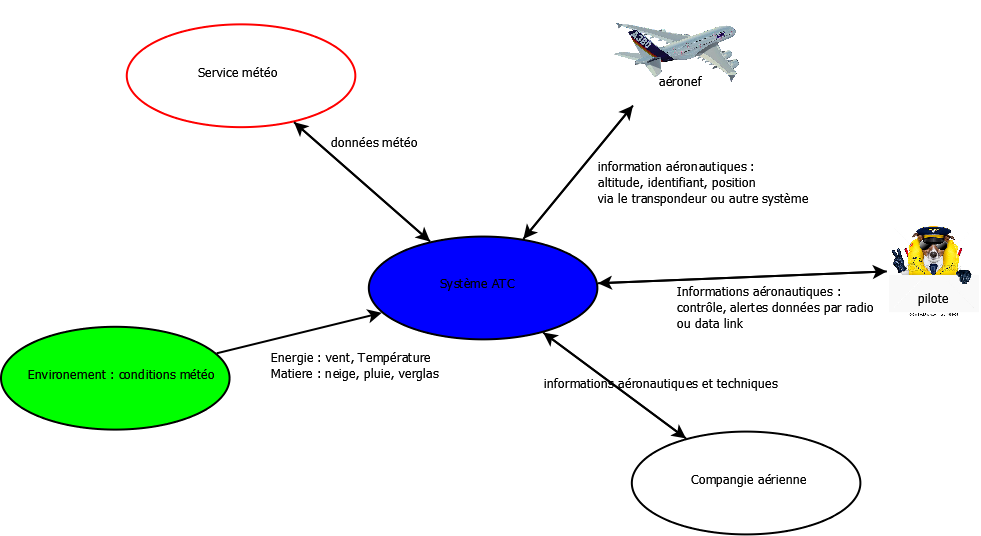
\includegraphics[scale=0.35]{images/ctx}
		\caption{Diagramme de contexte du système ATC}
		\label{ctx}
	\end{center}
\end{figure}

\subsection{ Description graphique du méta-modèle }

Les fonctions, les items et les composants sont les principaux éléments du méta modèle de la  figure \ref{meta}. En particulier, une fonction peut recevoir en entrée, ou fournir en sortie, un item information ou être déclenchée par un item signal électrique. La classe Requirement est intéressante dans le sens où elle permet de vérifier que les exigences sont toutes "mapées" avec un fonction qu'elle spécifie. 

\begin{figure}[H]
	\begin{center}	
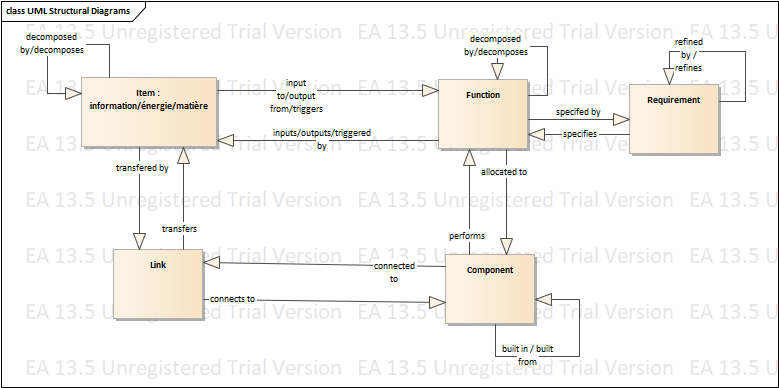
\includegraphics[scale=0.50]{images/meta_modele}
\caption{meta modèle Vitech core}
\label{meta}
	\end{center}
\end{figure}


\subsection{ Données manipulées }

Les données manipulées sont les suivantes :
\begin{itemize}
	\item L'identifiant issu du plan de vol ou d'un radar secondaire,
	\item La position de l'aéronef.
\end{itemize}

La position d'un aéronef vu par un radar primaire ne donne que la distance et l'azimut. Les radars secondaires donnent en outre l'altitude et l'identifiant de l'appareil. Les positions radar doivent être converties en longitude/latitude WGS84 pour pouvoir être affichées. Ce dernier point n'a pas été pris en compte explicitement dans le modèle. En outre, le modèle CORE
ne distingue pas clairement entre position 2D des radars primaires et 3D des radars secondaires ; les fonctions de traitements spécifiques, ainsi que d'autres fonctions, ont été supprimées pour limiter la taille des  graphes hiérarchiques et EFFBD. Ceci constitue un écart par rapport au cahier des charges de l'énoncé mais reste dans l'esprit de l'exercice.

\section{Aspect fonctionnelle}
	
	\subsection{Décomposition fonctionnelle}
	
	L'analyse du sujet a conduit à quatre fonctions principales décomposées en sous-fonctions selon le diagramme hiérarchique de la figure \ref{hier} :
	
	\begin{itemize}
		\item Acquérir les informations, 
		\item Traiter les informations,
		\item Afficher les informations,
		\item Communiquer
	\end{itemize}

L'analyse du modèle a mis en évidence, s'il était besoin, le rôle crucial
de la communication entre contrôleur et pilote dans la fourniture du service de contrôle, d'alerte et de surveillance. Sur le plan métier, la radio comme moyen de communication constitue le maillon faible des systèmes ATC actuel. En ce sens, la modélisation permet 
de mettre en évidence des failles du domaine réel ce qui constitue une source de progrès. 
	
	\begin{figure}[H]
		\begin{center}	
			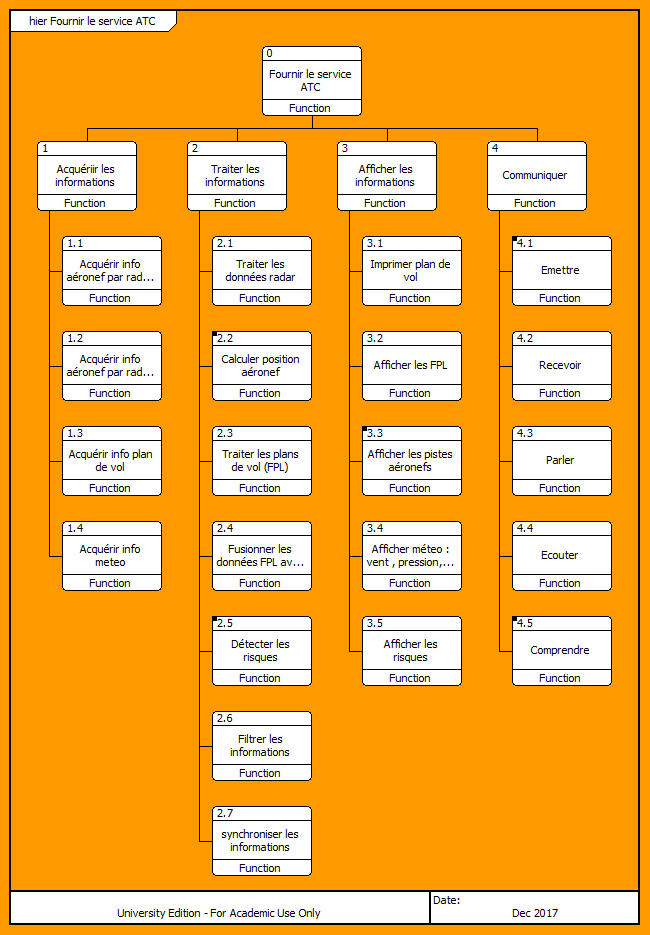
\includegraphics[scale=0.85]{images/hierarchique}
			\caption{Diagramme hiérarchique des fonctions}
			\label{hier}
		\end{center}
	\end{figure}
	
	\subsection{Scénario fonctionnel}

    Les diagrammes d'activités, EFFBD ou de séquence permettent de capturer un ou plusieurs scenarii du système modélisé. La démarche utilisée a consisté à créé un diagramme EFFBD dans CORE en utilisant uniquement les fonctions feuille puis de travailler sur le diagramme N2 pour l'ajout des items. Un exemple est donné en figure \ref{atc}. Le scénario associé à l'ensemble des fonctions feuille se trouve à l'adresse  \url{https://github.com/kad15/AF/blob/master/LIVRABLES_ATC_YUAN_BELDJILALI/question%207%20%20scenario%20fonctionnel%20unique.png}
    
    	\begin{figure}[H]
    	\begin{center}	
    		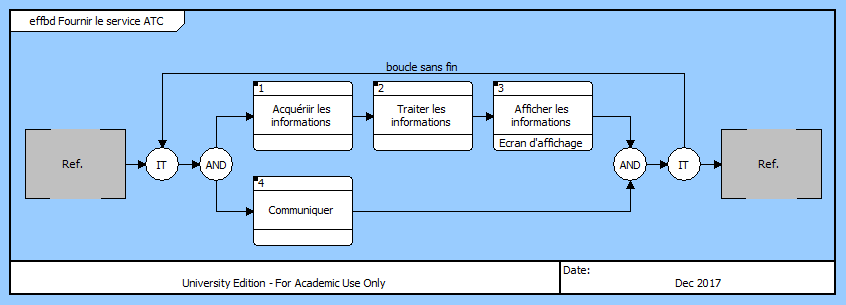
\includegraphics[scale=0.75]{images/atc}
    		\caption{Diagramme EFFBD simplifié du service ATC}
    		\label{atc}
    	\end{center}
    \end{figure}
    

\section{Rôle de l'ATM dans le futur par rapport aux stratégies des acteurs }

L'\textit{Air Traffic Management} est un domaine en perpétuelle évolution, tout particulièrement ces dernières années en Europe. En effet, il s'agit d'un secteur où les procédures et les outils doivent évoluer et s'adapter au trafic afin d'assurer une meilleure gestion du trafic tout en gardant un niveau de sécurité élevé. Nous allons voir un certain nombre d'évolutions qui pourraient avoir un impact sur les acteurs du fret aérien.

\subsection{L'opportunité du programme SESAR}

Comme le montre \cite{52008DC0750}, le programme \textit{Single European Sky ATM Research} (SESAR) mis en place par la Commission Européenne affiche d'ambitieux objectifs tels que :
\begin{itemize}
\item une réduction de moitié des coûts de contrôle aérien;
\item une réduction de 10\% de l'impact sur l'environnement;
\item une division du risque d'accident par 10;
\item un triplement de la capacité de l'espace aérien.
\end{itemize}

Dans ce contexte, les entreprises de fret aérien, au même titre que l'ensemble des compagnies aériennes volant en Europe, vont voir apparaitre la possibilité d'augmenter leurs capacités et de diminuer leurs coûts. Ainsi, si les échanges commerciaux continuent à croitre, notamment avec l'Asie, ces entreprises de transport pourront se développer sans contraintes immédiates dues à la gestion du trafic aérien.

Ces objectifs pourront être rendus possibles par le progrès technique (moteurs plus économiques et moins bruyants), la généralisation de procédures efficaces (descente continue) et la refonte du ciel européen qui souffre aujourd'hui d'une coûteuse segmentation et d'un manque d'harmonisation et de standardisation.\\

On voit donc en quoi les travaux actuels de modernisation de l'ATM permettent d'ouvrir un certain nombre de perspectives aux entreprises de transport aérien en général et, par conséquent, aux entreprises de transport aérien de fret en particulier.

\subsection{Introduction de nouveaux paradigmes}

Dans le cadre des réflexions relatives à la privatisation de certains ANSP (\textit{Air Navigation Service Provider}), des idées de services commerciaux que pourraient vendre ces entités ont émergé.

Par exemple, il serait envisageable de moduler le tarif de la redevance de contrôle en fonction du gain de temps ou du retard que serait prête à accepter une compagnie. Ainsi, une compagnie qui souhaiterait être prioritaire sur l'attribution d'un créneau paierait une redevance plus élevée qu'une compagnie prête à accepter un retard.

Or nous avons pu voir que l'une des spécificités du transport aérien de fret est que les marchandises sont, dans le cas général, résilientes face aux retards. Ainsi, grâce à ces services commerciaux liés à la gestion du trafic, les transporteurs aériens de fret pourraient optimiser leurs coûts dans certains cas.\\

On voit donc que de nouveaux paradigmes émergent au sein des ANSP et que ceux-ci peuvent impacter fortement la stratégie des transporteurs aérien de fret.

\subsection{Vers une extension du périmètre du fret}

%Etablissement de régulation lors du développement des drônes et avions sans pilotes : voilure mobile ou fixe. 

Comme le montre \cite{RePEc:eee:jaitra:v:61:y:2017:i:c:p:34-40}, de nouvelles entrées, certes limitées mais réelles, font leur apparition sur le marché du transport aérien de fret. Il s'agit principalement d'opérateurs de drones souhaitant réaliser un transport de marchandise par le biais de cette nouvelle technologie.

On peut citer notamment des entreprises comme La Poste \cite{gradt_2016} ou Amazon \cite{figaro_2016} qui tentent de mettre en place ce nouveau marché.

Si ce nouveau segment répond plutôt à la problématique du dernier kilomètre qui ne concerne pas tous les acteurs du transport aérien de fret, il est à noter que les évolutions de l'ATM vont jouer un rôle essentiel dans le développement de ce marché.

En effet, l'automatisation du transport aérien de marchandise pose un grand nombre de difficultés au regard de la gestion du trafic aérien dans certains espaces. De nouveaux concepts émergent alors : on parle ainsi de l'UTM (\textit{Unmanned Aircraft Systems} (UAS) \textit{Traffic Management}) au lieu de l'ATM pour désigner ces problématiques de gestion de trafic propres aux drones.\\ 

Ainsi, les évolutions technologiques dans les domaines de l'ATM, de l'UTM et des drones apporteront de nouvelles possibilités de développement aux acteurs du transport aérien de marchandises.






\section*{Conclusion}
\addcontentsline{toc}{section}{Conclusion}


\paragraph{}
La démarche employée est itérative. Dans l'approche MBSE, on divise le système en fonctions et sous fonctions que l'on confrontent d'un côté aux exigences si ces dernières ont été saisie dans CORE et de l'autre aux composants qui assurent ces fonctions. Le tracé de diagrammes dynamiques comme les EFFBD aident à visualiser le système en action et donc à découvrir des fonctions qu'on auraient pu oublier et à régler le niveau de granuralité optimal au même titre que le reporting permis par CORE qui confronte fonctions, composant, item, link.  

\paragraph{}
Le reporting de CORE est aussi une aide précieuse pour la validation du projet en amont par le client et l'évaluation financière et ressources nécessaires à ce dernier.

\paragraph{}
Par manque de temps, les aspects link et requirement n'ont pu être traités. Mais, ils n'étaient pas explicitement demandés. Il manque de plus à ce projet encore de nombreuses itérations ; la précipitation est génératrice de bugs. Enfin, l'aspect maintien en conditions opérationnelles du système ATC n'a pas été abordé, celui du développement de ces systèmes non plus.

\paragraph{}
CORE semble donc aider à construire "the right system and the system right". En particulier permet d'assurer
l'exhaustivité de la prise en compte des exigences par les fonctions. Encore faut-il que les exigences traduisent correctement les besoins.


%\newpage
%\appendix
%\section{Annexe}
\label{annexe_A}

\begin{itemize}
\item Pour écrire simplement les clés sur le disque, nous utilisons Marshal, qui garantit la compatibilité entre toutes les plateformes pour une même version de OCaml.
\item Bien que BatIO propose une API pour manipuler les canaux au niveau du bit, nous avons préféré rester au niveau de l'octet car il s'agit d'une solution plus évolutive – rares sont les bibliothèques proposant ce genre de fonctions. D'ailleurs, son fonctionnement est identique à ce que nous implémentons, reposant sur une lecture octet par octet.
\item Dans la version actuelle du code, les canaux d'entrées-sorties ne sont pas toujours fermés proprement lorsqu'une exception « fatale » est rencontrée…
\item Les blocs chiffrés sont écrits sur le canal de sortie sous forme de chaîne de caractères. Ainsi, le message chiffré constitué de deux blocs « 1234 5678 » est écrit, sous forme hexadécimale, «~31 32 33 34 00 35 36 37 38 00~». Pour déchiffrer, on lit donc le canal d'entrée « chaîne par chaîne ». Cela a l'avantage de produire une sortie lisible mais présente l'inconvénient de consommer bien plus d'espace qu'une représentation binaire qui serait spécialement conçue pour le problème.
\end{itemize}

%\section{Annexe}
\label{annexe_A}

\begin{itemize}
\item Pour écrire simplement les clés sur le disque, nous utilisons Marshal, qui garantit la compatibilité entre toutes les plateformes pour une même version de OCaml.
\item Bien que BatIO propose une API pour manipuler les canaux au niveau du bit, nous avons préféré rester au niveau de l'octet car il s'agit d'une solution plus évolutive – rares sont les bibliothèques proposant ce genre de fonctions. D'ailleurs, son fonctionnement est identique à ce que nous implémentons, reposant sur une lecture octet par octet.
\item Dans la version actuelle du code, les canaux d'entrées-sorties ne sont pas toujours fermés proprement lorsqu'une exception « fatale » est rencontrée…
\item Les blocs chiffrés sont écrits sur le canal de sortie sous forme de chaîne de caractères. Ainsi, le message chiffré constitué de deux blocs « 1234 5678 » est écrit, sous forme hexadécimale, «~31 32 33 34 00 35 36 37 38 00~». Pour déchiffrer, on lit donc le canal d'entrée « chaîne par chaîne ». Cela a l'avantage de produire une sortie lisible mais présente l'inconvénient de consommer bien plus d'espace qu'une représentation binaire qui serait spécialement conçue pour le problème.
\end{itemize}


\newpage
\nocite{*}  %affiche toutes les entrées du bib même celles qui ne sont pas citées.
% cf.    http://www.tuteurs.ens.fr/logiciels/latex/bibtex.html
% compilation en TROIS PHASE  bibtex traite un fichier *.aux mais bibtex mon_fichier comme bibtex mon_fichier.aux sont acceptés 
% latex mon_fichier.tex
% bibtex mon_fichier
% latex mon_fichier.tex


% \renewcommand{\bibname}{Toto}
% ou
%\renewcommand{\refname}{Bibliographie}
% dans le préambule.
%\bibliographystyle{alpha}
%\bibliography{references}
\pagebreak

\subsubsection*{}
\pagebreak
\thispagestyle{empty}
\ThisTileWallPaper{1.45\paperwidth}{1.0\paperheight}{images/ctrl1}
\addtolength{\wpXoffset}{-4.5cm}


\justify








\end{document}
